\section{Introduction}
\label{sec:intro}

Ref.~\cite{Abi:2020wmh} is an example reference...

\begin{figure}[htbp]
  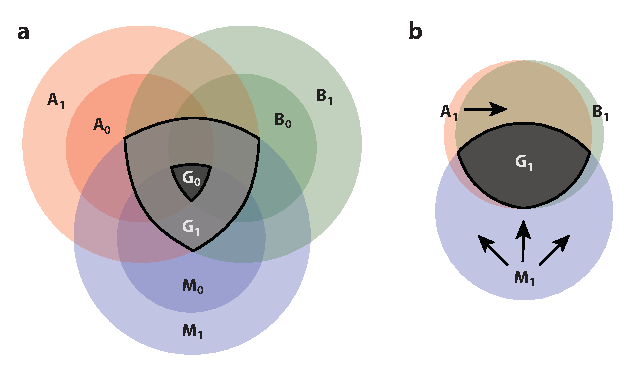
\includegraphics[width=0.6\textwidth]{plots/SampleFigure.eps}
  \caption{An example...}
  \label{fig:example}    
\end{figure}
Figure~\ref{fig:example} is an example...

The experimental neutrino oscillation program seeks to measure
 as of yet unknown properties associated with the change of flavor of neutrinos.
The mass hierarchy and CP violating phase of neutrinos still remain to be measured.
Measuring these quantities means stringent requirements on experimental precision.
High-intensity beams are required to produce the flux of neutrinos
 to be able to accumulate the necessary statistics.
Next generation neutrino oscillation experiments are of the billion dollar scale
 to meet these experimental constraints.

Two next-generation experiments are the Deep Underground Neutrino Experiment (DUNE)
 and the HyperKamiokande experiment (HyperK).
DUNE measures neutrinos over the first oscillation peak,
 corresponding to the range $1-10~{\rm GeV}$.
HyperK sits at lower energies peaking falling off after about $1~{\rm GeV}$.
At these energies, neutrino interactions with nucleons have many available interaction channels,
 including quasielastic, resonant, and deep inelastic scattering.
In order to increase the interaction cross section,
 large nuclear targets are used in place of elementary targets
 as both target and detection material.
Neutrino interaction cross sections on these large nuclear targets,
 and all of their complications,
 must be understood to make theoretical predictions about neutrino event rates.

Neutrino quasielastic scattering event topology is the simplest of these interactions
 since this interaction makes the assumption of scattering with a single free nucleon.
Despite the simplicity of this interaction,
 intranuclear rescattering of the particles can make the event topology observed
 in the detector more complicated.
Nuclear modeling is required to control these effects,
 which makes isolation of the initial free nucleon interaction more complicated.
In order to access the neutrino interaction cross sections with free nucleons,
 other methods must be employed.

The interaction via a weak current means that scattering cross sections are small,
 and so interaction data with elementary targets is sparse
 (in the case of bubble chamber experiments)
 or subject to uncontrollable model systematics
 (in the case of pion electroproduction experiments).
The dipole ansatz for the axial form factor is overconstrained
 and underestimates the form factor uncertainty by nearly an order of magnitude.
The nucleon axial form factor is poorly constrained from experimental data
 on elementary targets, with a 50\% uncertainty on the axial radius
 obtained from the model-independent $z$ expansion parameterization.
If the axial form factor uncertainty could be decreased,
 tensions in the neutron (?) magnetic form factor are still
 roughly half the size of the total axial form factor uncertainty,
 limiting the precision on the quasielastic neutrino-nucleon cross section.

Restrictions on new high-statistics bubble chamber experiemnts with
 hydrogen or deuterium fills are not likely due to safety considerations,
 so experiments are looking for other ways to access neutrino interactions
 with elementary targets.
One such way is to use experiments with various hydrocarbon targets
 and subtract away the carbon interaction contributions from
 the total hydrocarbon event rates.

In the absence of an updated scattering experiment on an elementary target,
 lattice QCD (LQCD) could provide the missing free nucleon amplitudes
 that are otherwise not known at the required precision.
The nucleon axial form factor is the first benchmark quantity that could be computed,
 with a few-${\rm GeV}^2$ reach in momentum transfer possible.
More challenging computations could provide information about nucleon
 resonant and nonresonant contributions to axial matrix elements,
 such as the $\Delta$ or Roper resonance channels,
 inclusive contributions in the shallow inelastic scattering region,
 or deep inelastic scattering parton distribution functions.

